\documentclass[11pt]{article}
\usepackage{amsmath}
\usepackage{graphicx}
\usepackage{subfig}
\usepackage{algorithmic}
\usepackage{algorithm}
\usepackage{relsize}
\usepackage{fancyhdr,authblk,multicol}
\usepackage{booktabs}

\title{\textbf{Symmetric Diffeomorphic Registration with Expected Cross-Correlation for Multi-Modal MRI}}
\date{}
%\author{Omar Ocegueda, Eleftherios Garyfallidis, \\Maxime Descoteaux and Mariano Rivera}
\author[a,*]{Omar Ocegueda}
\author[b]{Eleftherios Garyfallidis}
\author[b]{Maxime Descoteaux}
\author[a]{Mariano Rivera}

\renewcommand\Affilfont{\itshape\small}
\affil[a]{Centro de Investigacion en Matematicas, Guanajuato, Gto, Mexico}
\affil[b]{University of Sherbrooke, Quebec, Canada}

\begin{document}

\maketitle
\begin{abstract}
    We present an algorithm for Multi-Modal Symmetric Diffeomorphic Image Registration. The transfer functions between the two modalities are modeled as a set of
    hidden variables whose values are estimated using the Expectation Maximization (EM) algorithm. We apply the symmetric image normalization method (SyN) to
    maximize the image similarity defined by the transfer functions estimated in the E-step. We validate our algorithm using the publicly available IBSR database
    and the Brainweb synthetic template, obtaining very competitive results in both mono- and multi-modal image registration. Besides its simplicity, the EM
    Metric presents promising properties that can be exploited to design more sophisticated metrics. As a simple example, we extend the widely used Cross
    Correlation (CC) metric, which may not be used for multi-modality images in general. We show that our extension, Expected Cross Correlation (ECC),
    performs better than Cross Correlation in the multi-modal case, while being very competitive even in the mono-modal case.
\end{abstract}

\section{Introduction}

We regard an image $I$ as a function that maps voxels of a rectangular grid \hbox{$\mathcal{L} = \mathrm{Z}_{n_{x}} \times \mathrm{Z}_{n_{y}} \times \mathrm{Z}_{n_{z}}$} to a set $G$ of
possible values called the ``dynamic range'' of $I$. The images we are interested in represent objects in physical space. This means that each point $(i,j,k)$ in the
3-dimensional grid $\mathcal{L}$ is associated to a point $(x,y,z) \in \mathbf{R}^{3}$. When the coordinates of a point
\hbox{$(i,j,k)$} are not integers, the image can still be evaluated at $(i, j, k)$ by interpolation provided
\hbox{$(i,j,k) \in \left[0, n_{x}-1\right] \times \left[0, n_{y}-1\right] \times \left[0, n_{z}-1\right]$}, we denote this ``extended'' dense domain by using the bar decorator:
$\bar{\mathcal{L}}$.\\

The function that maps voxel coordinates of a grid $\mathcal{L}$ to their corresponding coordinates in physical space is an invertible affine transformation. Whenever we talk about
\textbf{a grid} $\mathcal{L}$ we implicitly assume that this $\mathcal{L}$ is associated to a specific grid-to-space affine transformation.
Since our images represent objects in physical space, and these objects are not tied to any specific grid, the same object may be \textbf{sampled} over any grid $\mathcal{L}$.
Note however that, if $\mathcal{A}$ is the grid-to-space affine transformation associated to $\mathcal{L}$, this grid can only sample objects contained in
$\Omega_{\mathcal{L}} = \mathcal{A}(\bar{\mathcal{L}}) \subset \mathbf{R}^{3}$. Since the grid-to-space transformation is invertible, we can, and will, unambiguously talk about the
value of image $I$ at a grid point $u\in \mathcal{L}$ or a point in space $u \in \Omega_{L}$.\\

A diffeomorphism is an invertible and differentiable function whose inverse is also differentiable. A diffeomorphism $\Psi$ is represented by a
deformation field $\phi$ that assigns a displacement vector $\phi(x)$ to each point $x$ such that $\Psi(x) = x + \phi(x)$ (therefore, the zero deformation field $\phi \equiv 0$
represents the identity diffeomorphism). The deformation field itself is defined in physical space and is discretized on its own grid, which of course is associated to
a grid-to-space transform.\\

Let $I, J$ be two images defined over grids $\mathcal{L}_{I}$, $\mathcal{L}_{J}$ with grid-to-space affine transforms $\mathcal{A}_{J}, \mathcal{A}_{I}$, respectively. Let
$\Psi:\Omega_{I} \rightarrow \Omega_{J}$ be a diffeomorphism where $\Omega_{I} = \mathcal{A}_{I}(\bar{\mathcal{L}_{I}})$,
and $\Omega_{J} = \mathcal{A}_{J}(\bar{\mathcal{L}_{J}})$ are the regions of $\mathbf{R}^{3}$ that are sampled by grids $\mathcal{L}_{I}$ and $\mathcal{L}_{J}$, respectively.
To ``warp'' image $J$ towards image $I$, we take each voxel $i \in \mathcal{L}_{I}$ and ``pull''the intensity value of $J$ at its corresponding point in $\mathcal{L}_{J}$
(fig. \ref{fig:pull_back}). More precisely, the warped image $\tilde{J}$ (denoted by the tilde decorator) under $\Psi$, is given by
\begin{equation}\label{eq:warp_definition}
    \tilde{J}(u) = J(\mathcal{A}_{J}^{-1}\Psi(\mathcal{A}_{I}u)), u \in \mathcal{L}_{I}
\end{equation}

\begin{figure}[H]
\centering
\fbox{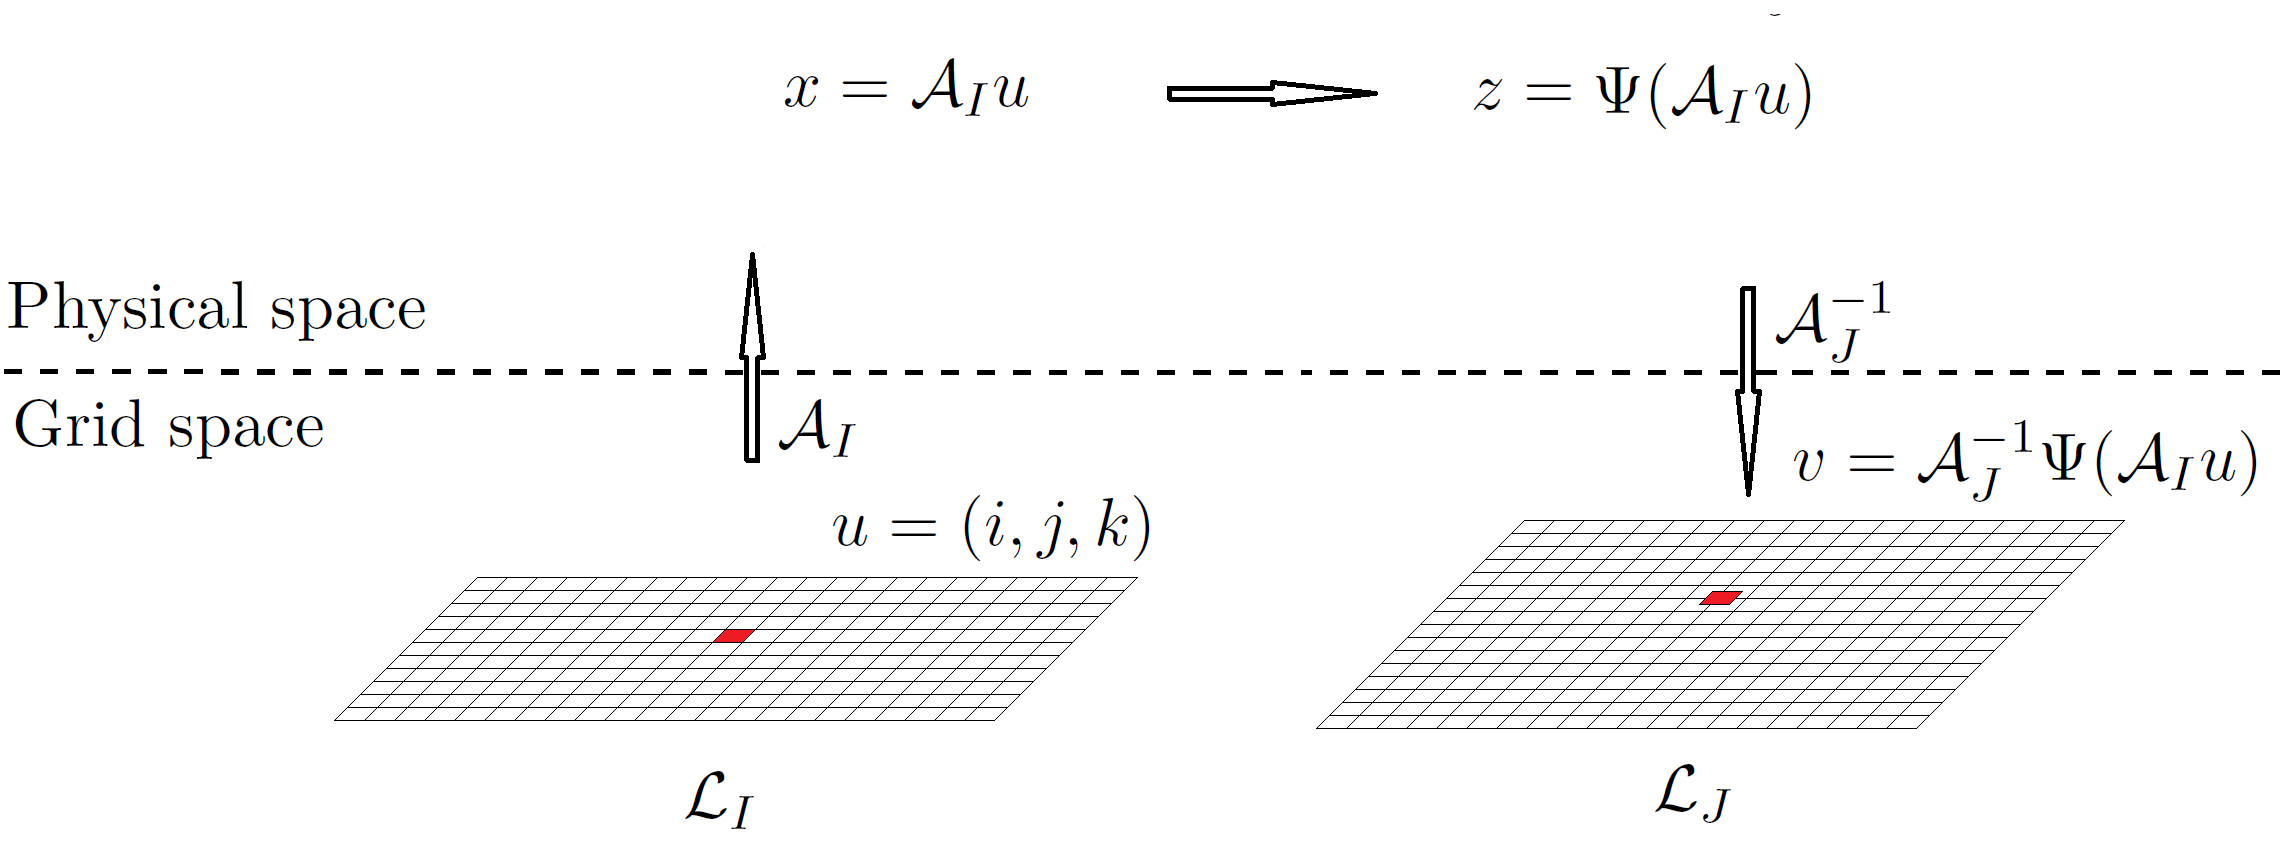
\includegraphics[width=1.0\linewidth]{./images/pull_back.png}}
\caption{Warping an image under a diffeomorphism $\Psi$ is accomplished by ``pulling'' image values at $\Psi$'s codomain towards its domain.}
\label{fig:pull_back}
\end{figure}

\subsection{Symmetric Normalization (SyN)}
The Symmetric formulation for Diffemorphic Image Registration proposed by Avants et al. \cite{Avants2009} consists in minimizing the variational energy given by:

\begin{equation}\label{eq:syn_energy}
    \begin{array}{lll}
        E(I, J) &=& \mathlarger{\int_{t=0}^{0.5} \left\lbrace ||v_{1}(x, t)||_{L}^{2} + ||v_{2}(x, t)||_{L}^{2}  \right\rbrace dt}\\
        &+&\mathlarger{ \int_{\Omega} P(I(\psi_{1}(0.5)), J(\psi_{2}(0.5)), x) d\Omega}
    \end{array}
\end{equation}
subject to
\begin{displaymath}
    \begin{array}{l}
        \frac{d\psi_{i}(x, t)}{dt} = v_{i}(\psi(x,t),t)\\
        \psi_{i}(x, 0) = Id, \psi_{i}^{-1}(\psi_{i}) = Id, \psi_{i}(\psi_{i}^{-1}) = Id, i=1,2,
    \end{array}
\end{displaymath}
where the norm $||\cdot||_{L}$ promotes regularity on the velocity fields $v_{i}$ by penalizing the result of applying the differential operator $L$ (choosen as
$L = \mu \nabla^{2} + \lambda Id$), and $P(I, J)$ is a metric
that measures the dissimilarity between images $I$ and $J$. The {\it symmetric normalization} (SyN) is defined as the solution of the above constrained optimization problem.
The algorithm proposed by Avants et al. \cite{Avants2009}, called {\it Greedy SyN} consists of an unconstrained search within the space of diffeomorphisms with homogeneous boundary
conditions. At each step, the Gready SyN algorithm updates the current estimate of $\psi_{1}, \psi_{2}$ by solving the Euler-Lagange equations defining necessary conditions
that the velocity fields $v_{i}$ must satisfy at each time to minimize eq. \ref{eq:syn_energy}. These equations were provided in \cite{Avants2006} for the Sum of Squared
Differences (SSD) metric as:
\begin{equation}\label{eq:euler_lagrange_ssd}
    Lv = (I - J)\nabla I.
\end{equation}

Equation \ref{eq:euler_lagrange_ssd} is important because it allows us to efficiently solve for $v$ by convolving $(I - J)\nabla I$ with the Green's kernel of the Laplacian $L$, which
is a Gaussian Kernel. Corresponding formulas to efficiently compute the update velocity fields driven by the Cross-Correlation metric were provided in \cite{Avants2009}.
Algorithm \ref{alg:Greedy_SyN} summarizes the Greedy SyN algorithm.

\begin{algorithm}[h!]
\caption{Greedy SyN}\label{alg:Greedy_SyN}
\begin{algorithmic}[1]
\STATE Greedy-SyN algorithm goes here
\end{algorithmic}
\end{algorithm}



\section{Extending SyN for multi-modality images}

Let $I$, $J$ be two images defined over the domains $\Omega_{I}$, $\Omega_{J}$, respectively. Let $G$ be the set of
possible intensity values these images may take (e.g. $G=\left\lbrace 0,1,...,255\right\rbrace$). Our objective is to find two diffeomorphisms
$\Psi_{I}:\Omega_{I}\rightarrow \Omega_{R}$, $\Psi_{J}:\Omega_{J}\rightarrow \Omega_{R}$ such that the images get aligned in the reference space $\Omega_{R}$
after warping them under $\Psi_{I}^{-1}$ and $\Psi_{J}^{-1}$. In other words, for each point $u \in \Omega_{R}$, $I(\Psi_{I}^{-1}(u))$ ``corresponds to'' $J(\Psi_{J}^{-1}(u))$
(fig. \ref{fig:syn_overview}). We will model the intensity correspondence between the two images as a set of hidden variables. More precisely, we will assume that there exist transfer functions
$F_{I}, F_{J}:G \rightarrow G$ such that:\\
\begin{equation}\label{eq:SyNEM_gom_ref}
    \begin{array}{ccccc}
        I(\Psi_{I}^{-1}(u)) &=& F_{J}[J(\Psi_{J}^{-1}(u))] &+& \eta_{J}(u)\\
        J(\Psi_{J}^{-1}(u)) &=& F_{I}[I(\Psi_{I}^{-1}(u))] &+& \eta_{I}(u)
    \end{array}, u\in\Omega_{R},
\end{equation}
where $\eta_{I}, \eta_{J}$ are independent random fields of independent random variables, i.e. $\eta_{I}(u) \perp \eta_{I}(v)$,
$\eta_{J}(u) \perp \eta_{J}(v)$ and $\eta_{I}(u) \perp \eta_{J}(v) \forall u,v\in \Omega_{R}$. By defining the warped images $\tilde{I}(u) = I(\Psi_{I}^{-1}(u))$
and $\tilde{J}(u) = J(\Psi_{J}^{-1}(u)), u \in \Omega_{R}$ we can write

\begin{figure}[H]
\centering
\fbox{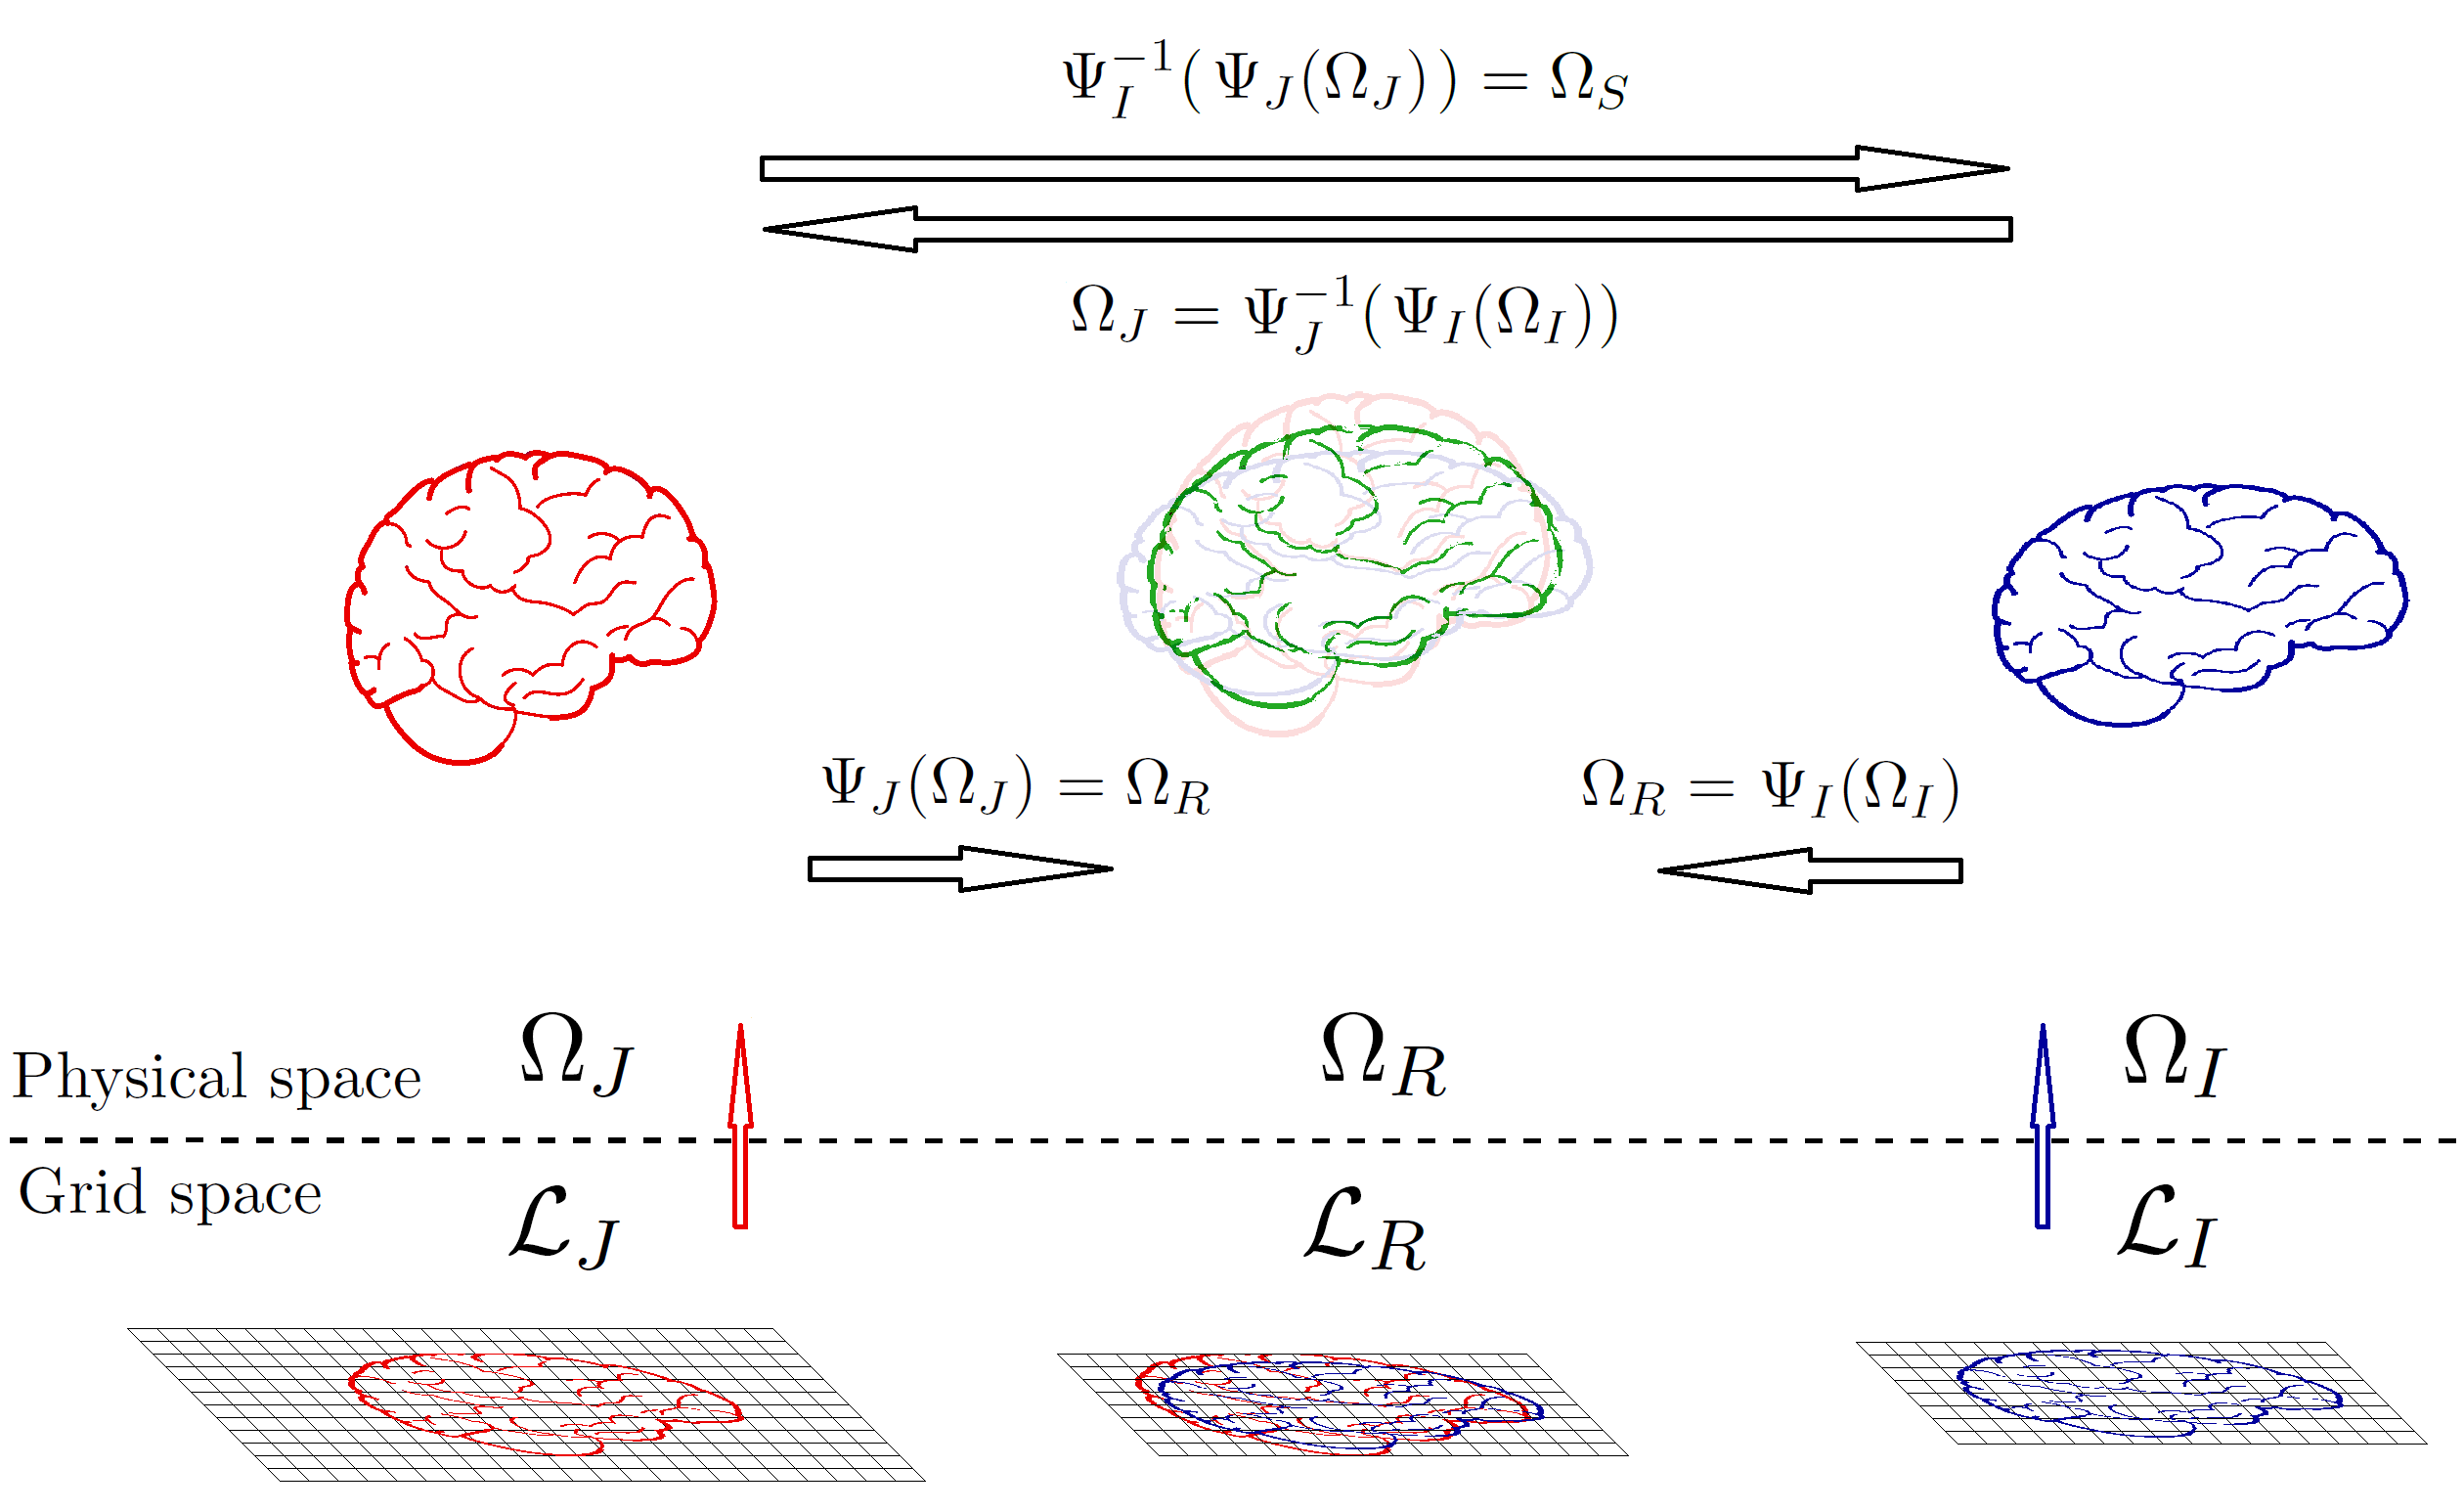
\includegraphics[width=1.0\linewidth]{./images/syn_overview.png}}
\caption{The SyN algorithm registers two input images by computing two diffeomorphisms that map the input images towards a common reference domain. The final
diffeomorphism is computed by composing the two partial diffeomorphisms.}
\label{fig:syn_overview}
\end{figure}

\begin{equation}\label{eq:SyNEM_gom_warped}
    \begin{array}{ccccc}
        \tilde{I}(u) &=& F_{J}[\tilde{J}(u)] &+& \eta_{J}(u)\\
        \tilde{J}(u) &=& F_{I}[\tilde{I}(u)] &+& \eta_{I}(u)
    \end{array}, u\in\Omega_{R},
\end{equation}
and now, both images are defined on the reference space. If we assume $\Psi_{I}$ and $\Psi_{J}$ are initial approximations to the true transformations
aligning $I$ and $J$, we are interested in computing two update diffeomorphisms (endomorphisms) \hbox{$\psi_{I}, \psi_{J} : \Omega_{R} \rightarrow \Omega_{R}$} such that

\begin{equation}\label{eq:SyNEM_gom_update}
    \begin{array}{ccccc}
    	\tilde{I}(\psi_{I}(u)) &=& F_{J}[\tilde{J}(u)] &+& \eta_{J}(u)\\
        \tilde{J}(\psi_{J}(u)) &=& F_{I}[\tilde{I}(u)] &+& \eta_{I}(u)
    \end{array}, u\in\Omega_{R}.
\end{equation}

By introducing the (unknown) sets of hidden variables $Y = \left\lbrace Y_{g}=F_{I}[g] : g\in G \right\rbrace$, $Z = \left\lbrace Z_g = F_{J}[g] : g \in G\right\rbrace$ we may
apply the EM algorithm to iteratively maximize the posterior distribution
$P(\Psi | \tilde{I}, \tilde{J}) = \frac{P(\tilde{I}, \tilde{J} | \Psi)P(\Psi)}{P(\tilde{I}, \tilde{J})}$ with respect to the transformations
$\Psi = (\psi_{I}, \psi_{J})$. The estimated diffeomorphisms at iteration $t$, $\Psi^{t} = \left( \psi_{I}^{t}, \psi_{J}^{t}\right)$ can be obtained from those at iteration
$t-1$ by maximizing, with respect to $\Psi$:
\begin{equation}
	Q(\Psi, \Psi^{t-1}) = E_{Y,Z}\left[\log \left( \frac{P(\tilde{I}, \tilde{J}, Y, Z|\Psi)P(\Psi)}{P(\tilde{I}, \tilde{J}, Y, Z)}\right) | \tilde{I}, \tilde{J}, \Psi^{t-1}\right].
\end{equation}
To evaluate this expected value, we need to integrate over all possible realizations $y, z$ of the hidden variables $Y, Z$ with respect to the conditional distribution $P(y,z| \tilde{I}, \tilde{J}, \Psi^{t-1})$:
\begin{equation}\label{eq:expected_value}
Q(\Psi, \Psi^{t-1}) = \int_{y,z} (U(\Psi, y, z) - K_1)dP(y,z| \tilde{I}, \tilde{J}, \Psi^{t-1})
\end{equation}
where $K_{1} =\log P(\tilde{I}, \tilde{J}, Y, Z)$ is a normalization constant (does not depend on $\Psi$) and
\begin{align}\label{eq:SyNEM_objective}
	U(\Psi, y, z) = \log P(\tilde{I}, \tilde{J}, y, z|\Psi) + \log P(\Psi)=\\
    \nonumber\sum_{g\in G} \sum_{x : \tilde{I}(x) = g} -\frac{\left(y_g - \tilde{J}(\psi_{I}(x))\right)^{2}}{\sigma_{I}(g)^{2}} + \lambda R(\psi_{I})+\\
    \nonumber\sum_{g\in G} \sum_{x : \tilde{J}(x) = g} -\frac{\left(z_g - \tilde{I}(\psi_{J}(x))\right)^{2}}{\sigma_{J}(g)^{2}} + \lambda R(\psi_{J}).
\end{align}
The regularization functional $R(\cdot)$ encode our prior knowledge about $\Psi$ by $\log P(\Psi) = \lambda \left( R(\psi_{I}) + R(\psi_{J})\right)$ where $\lambda > 0$ is a parameter controlling the amount of regularization.\\

If we assume $Y$ and $Z$ are independent, and their elements $Y_g$ and $Z_g$, $g\in G$ are independent from each other, then the density function $P(y,z| I, J, \Psi^{t-1})$ can be written as the product of two separate densities
\begin{equation}\label{eq:density_products}
    P(y,z| I, J, \Psi^{t-1}) = h_{Y}(y)h_{Z}(z) = \prod_{g\in G}h_{Y_g}(y_g) \prod_{g\in G}h_{Z_g}(z_g),
\end{equation}
and the expected value (eq. \ref{eq:expected_value}) can be written as
\begin{align}
    -K_{1}-\int\sum_{g\in G} \sum_{x : I(x) = g} \frac{\left(y_g - \tilde{J}(\psi_{I}(x))\right)^{2}}{\sigma_{I}(g)^{2}}d h_{Y}(y)-\\
    \nonumber\int\sum_{g\in G} \sum_{x : J(x) = g} \frac{\left(z_g - \tilde{I}(\psi_{J}(x))\right)^{2}}{\sigma_{J}(g)^{2}}d h_{Z}(z)
\end{align}
which can be further simplified (by using eq. \ref{eq:density_products} to split the densities $h_{Y}(y)$ and $h_{Z}(z)$ as products of individual densities for each intensity $g \in G$) as
\begin{align}
    -K_{1}-\sum_{g\in G} \sum_{x : I(x) = g} \int\frac{\left(r - \tilde{J}(\psi_{I}(x))\right)^{2}}{\sigma_{I}(g)^{2}}d h_{Y_g}(r)-\\
    \nonumber\sum_{g\in G} \sum_{x : J(x) = g} \int\frac{\left(s - \tilde{I}(\psi_{J}(x))\right)^{2}}{\sigma_{J}(g)^{2}}d h_{Z_g}(s)
\end{align}
now let $\bar{r}(g)$ and $\bar{s}(g)$ be the expected value of $Y_g$ and $Z_g$ given $I, J, \Psi^{t-1}$ respectively, then
\begin{align}
    &\int\left(r - \tilde{J}(\psi_{I}(x))\right)^{2}d h_{Y_g}(r) = &\\
    &\nonumber \int\left(r - \bar{r}(g) + \bar{r}(g) - \tilde{J}(\psi_{I}(x))\right)^{2}d h_{Y_g}(r) = &\\
    &\nonumber \sigma^{2}_{I}(g) + \int\left(\bar{r}(g) - \tilde{J}(\psi_{I}(x))\right)^{2}d h_{Y_g}(r) = &\\
    &\nonumber \sigma^{2}_{I}(g) + \left(\bar{r}(g) - \tilde{J}(\psi_{I}(x))\right)^{2}&
\end{align}
because $h_{Y_g}$ is a density function and we are integrating over its entire domain. Analogously:
\begin{align}
    \int\left(s - \tilde{I}(\psi_{J}(x))\right)^{2}d h_{Z_g}(s) = \sigma^{2}_{J}(g) + \left(\bar{s}(g) - \tilde{I}(\psi_{J}(x))\right)^{2}
\end{align}

Now let's denote by $\hat{\mu}_{I}(x) = \bar{r}(\tilde{I}(x))$, $\hat{\sigma}_{I}(x) = \sigma_{I}(\tilde{I}(x))$ and analogously
$\hat{\mu}_{J}(x) = \bar{s}(\tilde{J}(x))$, $\hat{\sigma}_{J}(x) = \sigma_{J}(\tilde{J}(x))$, in other words, we assign to each voxel $x$ from
$\tilde{I}$ the expected value $\bar{r}(g)$ corresponding to the intensity $g$ of $\tilde{I}$ at $x$ and denote it by $\hat{\mu}_{I}(x)$, assign
its corresponding variance and denote it by $\hat{\sigma_{I}}(x)$ and proceed analogously for $\hat{\mu}_{J}(x)$ and $\hat{\sigma}_{J}(x)$ using $J$.
Then, the expected value that needs to be maximized in the M-step of the EM algorithm (eq. \ref{eq:expected_value}) can be written as:
\begin{align}\label{eq:SyNEM_objective}
    -Q(\Psi, \Psi^{t-1}) = \sum_{x \in \Omega_{I}} \frac{(\hat{\mu}_{I}(x) - \tilde{J}(\psi_{I}(x)))^{2}}{\hat{\sigma}_{I}(x)} + \lambda R(\psi_{I}) + \\
    \nonumber\sum_{x \in \Omega_{J}} \frac{(\hat{\mu}_{J}(x) - \tilde{I}(\psi_{J}(x)))^{2}}{\hat{\sigma}_{J}(x)} + \lambda R(\psi_{J})
\end{align}

The main difficulty of directly minimizing eq. (\ref{eq:SyNEM_objective}) is that both similarity terms depend on both diffeomorphisms
$\psi_{I}$ and $\psi_{J}$ since $\tilde{J}(\psi_{I})$ depends on $\psi_{J}^{-1}$ and $\tilde{I}(\psi_{J})$ depends on $\psi_{I}^{-1}$, which implies that the
objective function must be optimized with respect to both diffeomorphisms simultaneously, which is very challenging because an explicit formula for the representation
of $\psi_{I}^{-1}$ and $\psi_{J}^{-1}$ in terms of the parameters of $\psi_{I}$ and $\psi_{J}$ may not be available or may be prohibitively costly to compute
\footnote{Diffeomorphisms are typically parameterized by displacement fields (a displacement vector for each voxel) and the problem of inverting a displacement field
has been subject of substantial research. All available methods for approximating displacement field inverses are iterative, see for example:
\cite{Chen2008}\cite{Avants2009}\cite{Christensen2001}\cite{Crum2007}\cite{Yan2010}}. To overcome this difficulty, the greedy SyN algorithm proposed by Avants et al.
\cite{Avants2011} uses the inverses at iteration $t-1$ to compute $\tilde{I}$ and $\tilde{J}$, then updates the direct transformations at iteration $t$ and updates the
inverses at iteration $t$ by inverting $\psi_{I}^{t}$ and $\psi_{J}^{t}$ using a variation of the fixed point algorithm proposed by Chen et al.\cite{Chen2008} (see
algorithm \ref{alg:SyNEM}). This scheme has the extra advantage that both similarity terms are now decoupled.\\



\begin{algorithm}[h!]
\caption{SyN-EM}\label{alg:SyNEM}
\begin{algorithmic}[1]
\REQUIRE Two images $I_{2}$, $I_{2}$
\REQUIRE Maximum number of iterations $M$
\REQUIRE Energy derivative tolerance $\tau$
\REQUIRE Number of quantization levels $q$

\medskip
\STATE $t = 0$
\STATE Initialize the displacement fields $\phi_{1}^{(t)}(x) = 0$, $\phi_{2}^{(t)}(x) = 0$
\REPEAT
    \STATE $t \leftarrow t+1$
    \STATE Warp the input images to the reference space $\tilde{I}_{1}(\cdot) = I_{1}(\psi_{I}^{-1(t-1)}(\cdot))$, $\tilde{I}_{2}(\cdot) = I_{2}(\psi_{J}^{-1(t-1)}(\cdot))$
    \STATE Solve for $\phi_{1}^{*}$, $\phi_{2}^{*}$
    \STATE Compose $\psi_{I}^{t}(\cdot) = \psi_{i}^{*}(\psi_{i}^{t-1}(\cdot))$
    \STATE Update the inverses at iteration t
\UNTIL{$t \geq M$ \OR $\epsilon<\tau$}
\STATE Compute the forward transform: $\psi = (\psi_{2}^{t})^{-1} \circ \psi_{1}^{t}$
\STATE Compute the backward transform: $\psi^{-1} = (\psi_{1}^{t})^{-1} \circ \psi_{2}^{t}$
\RETURN $\psi$, $\psi^{-1}$
\end{algorithmic}
\end{algorithm}


\section{Gauss-Newton Step}

\section{Demons Step}
After modeling the transfer function from voxel intensities in the static image to voxel intensities in the moving image, we obtain the following energy function that needs to be minimized to obtain the optimal displacement filed (eq. 22 of \cite{Arce-santana2014}):

\section{Experiments}
\subsection{Mono-modal registration}

In the first experiment we will follow the methodology of Rohlfing et al.\cite{Rohlfing2012}, which consists on registering all 18 T1 brains from the publicly available IBSR database against each other, resulting in 306 registrations. We evaluate the accuracy of the registration by computing the Jaccard index over 31 anatomical regions manually annotated on the T1 brain images.

[Conclusion: SyNEM is very competitive, it compares favourably to FFD (one of the best performers in Klein's study \cite{Klein2009}) but still not as good as SyN with cross correlation. This may be explained by the fact that CC uses a relatively large window centered at each voxel for computing the similarity, while the EM is voxelwise, however, note that even if the images are T1 monomodal, a naive registration using SSD is not enough because of the spatial inhomogeneities and differences in the intensity spectrum of the images (show a pair of images as an example), show the result using SSD. So, a pre-processing is necessary to match the histograms (show the results using match-histogram from ANTS), but SyNEM compares favourably against SSD with some bias correction (try the bias correction algorithm by Tustison et al.). We conclude that SyNEM is able to handle differences in the intensities of monomodal images, and partly correct bias field inhomogeneities. However it is not the best option for monomodal registration (cross correlation performs better).]

\subsection{Multi-modal registration}
It is a common practice within the neuroimaging community to use the cross-correlation metric to register T1 vs T2 brain MRI images. The argument in favor of using
this metric is that these modalities are related by an ``almost linear'' transfer function. To illustrate the danger of doing this, we used the Brainweb synthetic
template [citation needed]. Brainweb provides two perfectly aligned, realistically simulated brain MRI in T1 and T2 modalities. Ideally, a multi-modal registration method
should return the identity transformation to register these perfectly aligned images.

\begin{figure}[H]
\centering
\fbox{\subfloat[Brainweb T1 (left) and T2(right) overlaid using two different channels(middle). T1 is depicted in red and T2 in green.]{\label{fig:brainweb_t1_t2_input}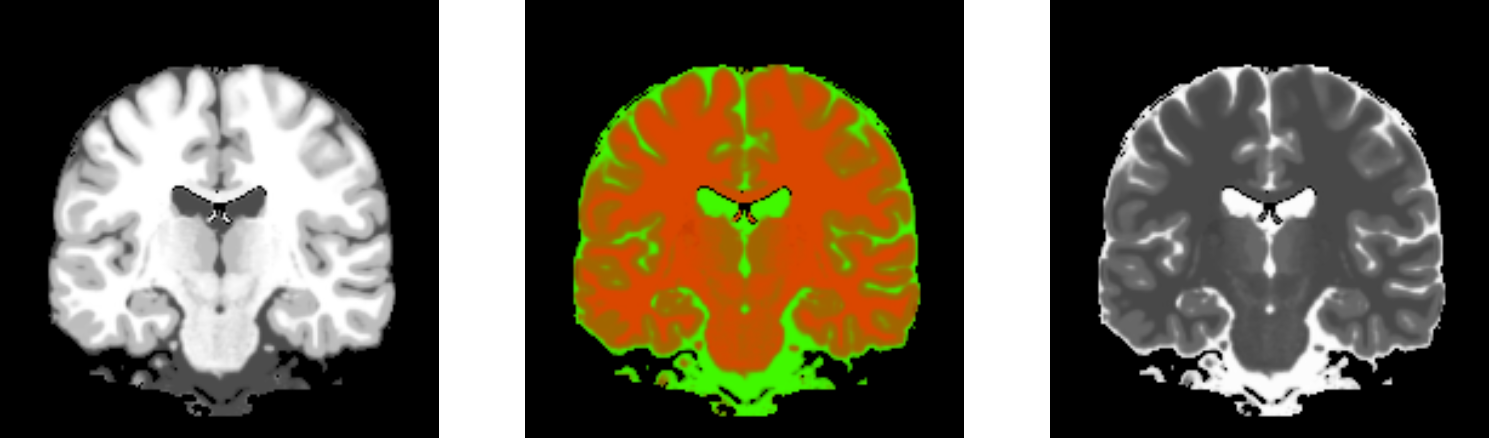
\includegraphics[width=1.0\linewidth]{./images/brainweb_t1_t2_overlay.png}}}\\
\fbox{\subfloat[T2 registered towards T1 using ANTS with the Cross-Correlation metric. Boundaries are clearly distorted.]{\label{fig:syncc_brainweb_t1_t2_overlay}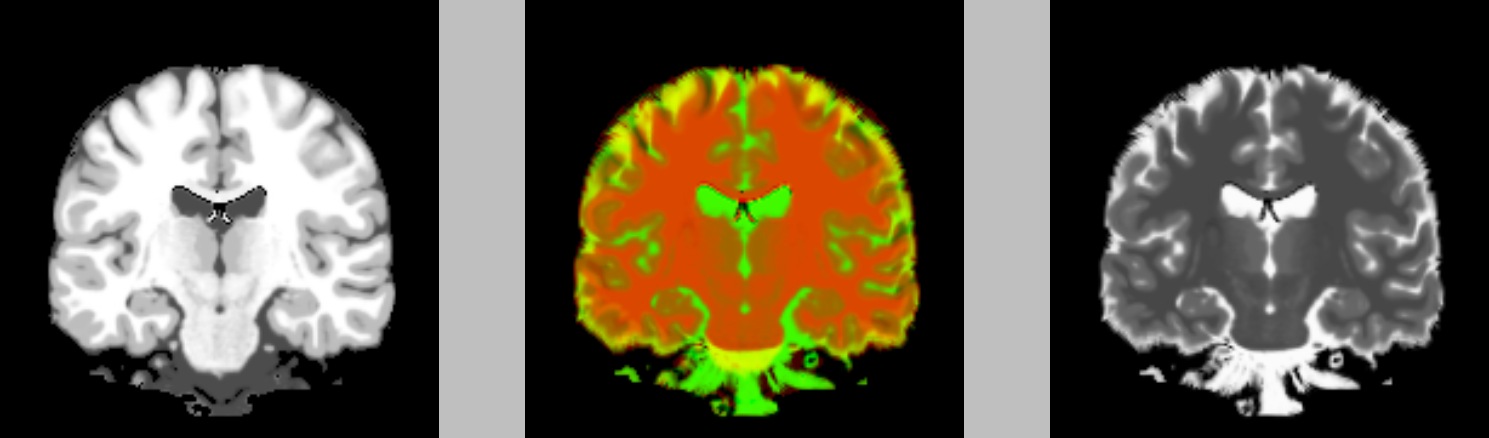
\includegraphics[width=1.0\linewidth]{./images/syncc_brainweb_t1_t2_overlay.png}}}
\fbox{\subfloat[T2 registered towards T1 using SyN algorithm with the Expected Cross-Correlation metric. Deformations are hard to see: ventricles are slightly dilated.]{\label{fig:syencc_brainweb_t1_t2_overlay}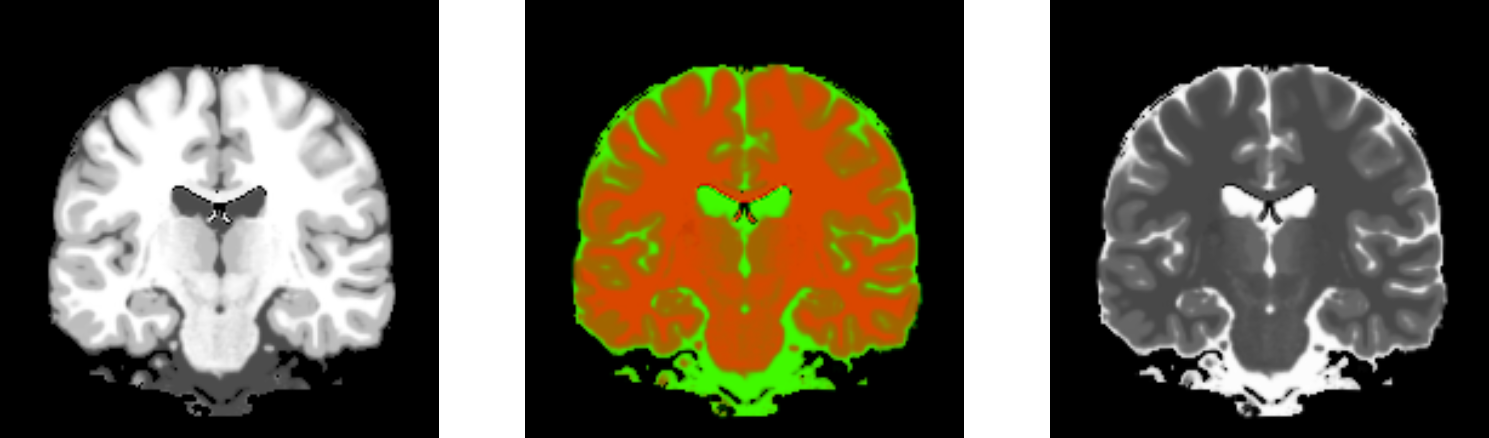
\includegraphics[width=1.0\linewidth]{./images/synecc_brainweb_t1_t2_overlay.png}}}
\caption{Registration of two perfectly aligned images with different modalities.}
\label{fig:brainweb_t1_t2}
\end{figure}

The analog to Klein's experiment for multi-modality data would register manually annotated images from two different modalities and use the Jaccard indices to measure
registration accuracy. Unfortunately, to the best of our knowledge, there are no manually annotated multi-modality data publicly available, so we will perform a less
realistic experiment using the Brainweb synthetic template [citation needed]. Brainweb provides two perfectly aligned, realistically simulated brain MRI in two modalities
T1 and T2. We generated synthetic T2 images for all IBSR T1 images by first registering the Brainweb T1 image (which plays the role of moving image) towards each IBSR
T1 image (which play the role of static image) using ANTS. Then we applied the obtained deformation field to the Brainweb T2 image and computed the transfer function
from T1 to T2 intensities and applied the transfer function to the IBSR T1 obtaining a ``perfectly aligned'' realistic synthetic T2 image for each IBSR volume, therefore
the annotations remain exactly the same as the T1 counterparts and we are able to execute Rholfing's experiment but this time using different modalities. Note that the number
of registrations we need to perform is now 612 because we can use the T2 modality either as the moving or the static image.\\



Being a synthetic template, it is possible to generate two perfectly registered images of different modalities
(T1 and T2). The Brainweb template is
not annotated into the same anatomical areas as the IBSR database, so we cannot directly measure the accuracy of registration of the IBSR images to the template, but we
can measure the sensitivity of the registration methods to the change of modality. In other words, if we register one arbitrary T1 image from IBSR to the T1 image of the
Brainweb template (mono-modal case) we should obtain exactly the same registration result if we register the same IBSR image to the T2 image of the Brainweb template
(multi-modal case) if the registration algorithm correctly handles the multi-modality.

% Table generated by Excel2LaTeX from sheet 'SyNEM-Multi-Large'
\begin{table}[htbp]
  \centering
  {\small
    \begin{tabular}{rrrr}
    \toprule
          & \textbf{SyN-ECC} & \textbf{SyN-EM} & \textbf{SyN-CC} \\
    \midrule
    \textbf{Right-Thalamus-Proper:} & \textbf{0.758} & 0.716 & 0.756 \\
    \textbf{Left-Thalamus-Proper:} & \textbf{0.754} & 0.727 & 0.752 \\
    \textbf{Left-Lateral-Ventricle:} & 0.709 & 0.706 & \textbf{0.733} \\
    \textbf{Right-Lateral-Ventricle:} & 0.696 & 0.687 & \textbf{0.718} \\
    \textbf{Left-Putamen:} & \textbf{0.740} & 0.699 & 0.683 \\
    \textbf{Right-Putamen:} & \textbf{0.742} & 0.684 & 0.676 \\
    \textbf{Brain-Stem:} & \textbf{0.790} & 0.786 & 0.663 \\
    \textbf{Left-Cerebellum-Cortex:} & \textbf{0.765} & 0.729 & 0.649 \\
    \textbf{Right-Cerebellum-Cortex:} & \textbf{0.769} & 0.729 & 0.645 \\
    \textbf{Left-Caudate:} & \textbf{0.652} & 0.628 & 0.637 \\
    \textbf{Right-Caudate:} & \textbf{0.636} & 0.606 & 0.618 \\
    \textbf{Right-Cerebral-White-Matter:} & \textbf{0.723} & 0.683 & 0.571 \\
    \textbf{Left-Cerebral-White-Matter:} & \textbf{0.722} & 0.685 & 0.570 \\
    \textbf{Left-Cerebral-Cortex:} & \textbf{0.700} & 0.699 & 0.558 \\
    \textbf{Right-Cerebral-Cortex:} & \textbf{0.697} & 0.694 & 0.548 \\
    \textbf{4th-Ventricle:} & \textbf{0.583} & 0.546 & 0.543 \\
    \textbf{Right-Hippocampus:} & \textbf{0.610} & 0.570 & 0.503 \\
    \textbf{Right-VentralDC:} & \textbf{0.642} & 0.616 & 0.499 \\
    \textbf{Right-Pallidum:} & \textbf{0.606} & 0.528 & 0.499 \\
    \textbf{Left-Pallidum:} & \textbf{0.602} & 0.545 & 0.495 \\
    \textbf{3rd-Ventricle:} & \textbf{0.517} & 0.511 & 0.492 \\
    \textbf{Left-VentralDC:} & \textbf{0.640} & 0.622 & 0.491 \\
    \textbf{Left-Hippocampus:} & \textbf{0.600} & 0.567 & 0.488 \\
    \textbf{Left-Cerebellum-White-Matter:} & \textbf{0.688} & 0.582 & 0.485 \\
    \textbf{Right-Cerebellum-White-Matter:} & \textbf{0.690} & 0.579 & 0.476 \\
    \textbf{Left-Amygdala:} & \textbf{0.505} & 0.447 & 0.360 \\
    \textbf{Right-Amygdala:} & \textbf{0.497} & 0.415 & 0.339 \\
    \textbf{Right-Accumbens-area:} & \textbf{0.483} & 0.433 & 0.339 \\
    \textbf{Left-Accumbens-area:} & \textbf{0.494} & 0.448 & 0.338 \\
    \textbf{Left-Inf-Lat-Vent:} & \textbf{0.219} & 0.178 & 0.194 \\
    \textbf{Right-Inf-Lat-Vent:} & \textbf{0.219} & 0.164 & 0.178 \\
    \bottomrule
    \end{tabular}}%
    \caption{Comparison of the registration performance (measured by the Jaccard index over 31 anatomical regions) of the Greedy SyN algorithm with EM, ECC and CC metrics. The Jaccard
indices were averaged over 612 multimodal registrations. Top performer for each region is highlighted.}
  \label{tab:multimodal_results_seg}%
\end{table}%


% Table generated by Excel2LaTeX from sheet 'SyNEM-Multi-Large'
\begin{table}[htbp]
  \centering
  {\small
    \begin{tabular}{ccccc}
    \toprule
          & \textbf{SyN-EM} & \textbf{SyN-ECC} & \textbf{SyN-CC} & \textbf{SyN-MI} \\
    \midrule
    \textbf{Background} & 0.993 & 0.995 & 0.990 & \textbf{0.995} \\
    \textbf{CSF} & 0.275 & \textbf{0.335} & 0.157 & 0.325 \\
    \textbf{Gray Matter} & 0.718 & \textbf{0.742} & 0.597 & 0.691 \\
    \textbf{White Matter} & 0.685 & \textbf{0.718} & 0.572 & 0.622 \\
    \bottomrule
    \end{tabular}}%
  \caption{Comparison of the registration performance (measured by the Jaccard index over Background, CSF, GM and WM)of the Greedy SyN algorithm with EM, ECC, CC and MI metrics.
The Jaccard indices were averaged over 612 multimodal registrations. Top performer for each region is highlighted.}
  \label{tab:multimodal_results_segTri_fill}%
\end{table}%


\begin{figure}[H]
\centering
\label{fig:graph_seg}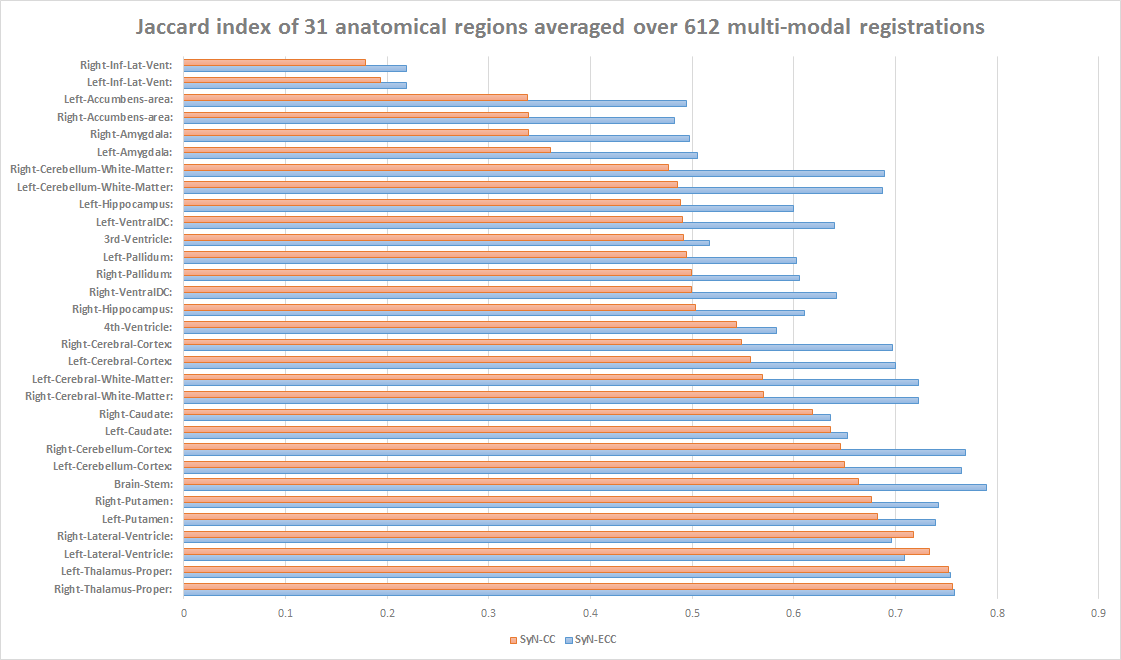
\includegraphics[width=1.0\linewidth]{./images/graph_seg.png}\\
\caption{Comparison of the registration performance (measured by the Jaccard index over 31 anatomical regions) of the Greedy SyN algorithm with CC and ECC.}
\end{figure}

\begin{figure}[H]
\centering
\label{fig:graph_segTri_fill}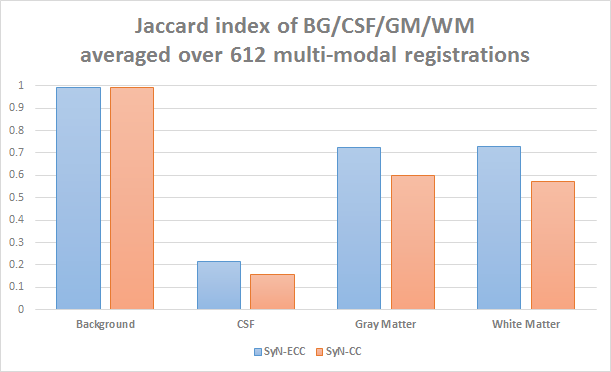
\includegraphics[width=1.0\linewidth]{./images/graph_segTri_fill.png}\\
\caption{Comparison of the registration performance (measured by the Jaccard index over Background, CSF, GM and WM)of the Greedy SyN algorithm with CC and ECC.}
\end{figure}

\bibliographystyle{plain}
\bibliography{references}

\end{document}


\section{Introduction}
Introduce the topic by splitting the proble into [a] The transformation model (and cite SyN as the state of the art for registration of brain MRI), and [b] The similarity metric (and cite information-theoretic similarity metric as the most successful for multi-modal registration)
Classical Multi-modal registration algorithms: \cite{Wells1996}\cite{Maes1997}

The image intensity associated to a tissue depends on the imaging modality (T1, T2, CT) and may even depend on geometric structure and other features of the tissue (FA, MD from diffusion MRI).


Correlation-based similarity metrics are designed for situations in which the image intensities of both images are linearly correlated and work well only for mono-modal images \cite{Roche2004}.

Our algorithm presents several extensions to the algorithm proposed by Arce et al. \cite{Arce-santana2014}: (1) our resulting deformation fields are diffeomorphic, (2) we estimate both transfer functions (static to moving and moving to static), (3) we derive a demons-like step to minimize the resulting energy function, which is more efficient and easier to implement [comment: we also have the Gauss-Newton step solving the large linear system using the multi-resolution algorithm (in addition to the Gaussian pyramid), may be we can submit a version using Gauss Newton and then another one using the demons-like step].

\section{The SyN algorithm}
[briefly explain the SyN algorithm as a greedy algorithm to find the diffeomorphisms at time 0.5 and state than we are going to denote such "mid-point" diffeomorphisms as $\psi_{1}$ and $\psi_{2}$. Also explain the role of the reference domain $\Omega_R$ and state that typically it is chosen to be $\Omega{1}$, the domain of the static image.]
